\documentclass[10pt]{article}
\usepackage[paperwidth=216mm,paperheight=270mm,margin=0mm]{geometry}
\usepackage{carousel-theme}
\pagestyle{empty}
\setlength{\parindent}{0pt}
\begin{document}

% 1 Cover
\setslide{1}
\pagecolor{Navy}

\begin{tikzpicture}[remember picture,overlay]
\fill[Blue] ([xshift=-32mm,yshift=-35mm]current page.north east) circle (58mm);
\fill[Cyan,opacity=.75] ([xshift=-4mm,yshift=18mm]current page.south west) circle (48mm);
\draw[White,opacity=.18,line width=1.2pt] ([xshift=18mm,yshift=-25mm]current page.north west) rectangle ([xshift=-18mm,yshift=25mm]current page.south east);
\node[anchor=north west,text width=168mm] at ([xshift=21mm,yshift=-40mm]current page.north west) {%
{\sffamily\bfseries\fontsize{31}{34}\selectfont\color{White}Engineering\\LaTeX Templates\par}
\vspace{7mm}
{\sffamily\fontsize{15}{20}\selectfont\color{White!88}A reusable documentation system for reports, technical presentations, and IEEE-style papers.\par}
\vspace{10mm}
\pill{OPEN-SOURCE ENGINEERING WORKFLOW}\quad\pill{LATEX + GIT + PDF}
};
\node[anchor=south west,text=White] at ([xshift=21mm,yshift=29mm]current page.south west) {\sffamily\bfseries\fontsize{12}{14}\selectfont Hossein Molhem};
\node[anchor=south east,text=White!85] at ([xshift=-21mm,yshift=29mm]current page.south east) {\sffamily\fontsize{9}{11}\selectfont Swipe to explore \faArrowRight};
\end{tikzpicture}
\newpage

% 2 Problem
\pagecolor{Mist}\setslide{2}
\vspace*{19mm}\hspace*{16mm}\begin{minipage}{184mm}
\slideheading{Strong engineering deserves strong documentation.}{Technical work often loses impact because the reporting system is rebuilt from scratch for every project.}
\vspace{10mm}
\begin{center}
\card{Blue}{\faRedo}{Repeated setup} \hspace{3mm}
\card{Cyan}{\faPuzzlePiece}{Inconsistent structure} \hspace{3mm}
\card{Green}{\faHistory}{Lost decisions}
\end{center}
\vspace{10mm}
\begin{tikzpicture}
\node[rounded corners=4mm,fill=White,draw=Line,inner sep=7mm,text width=168mm] {\sffamily\fontsize{13}{17}\selectfont\color{Ink}\textbf{The core problem:} equations, figures, tables, references, appendices, and review decisions are frequently managed as isolated files rather than as one controlled engineering system.};
\end{tikzpicture}
\end{minipage}\slidefooter
\newpage

%3 solution architecture
\pagecolor{White}\setslide{3}
\vspace*{18mm}\hspace*{16mm}\begin{minipage}{184mm}
\slideheading{One repository. Three reusable document systems.}{Each template provides a practical starting point while preserving consistent engineering structure and version history.}
\vspace{8mm}
\begin{center}
\begin{tikzpicture}[node distance=8mm]
\node[rounded corners=4mm,fill=Blue!8,draw=Blue!25,minimum width=50mm,minimum height=56mm,align=center,font=\sffamily\bfseries,text=Navy] (r) {ENGINEERING\\REPORT};
\node[rounded corners=4mm,fill=Cyan!9,draw=Cyan!28,minimum width=50mm,minimum height=56mm,align=center,right=of r,font=\sffamily\bfseries,text=Navy] (p) {TECHNICAL\\PRESENTATION};
\node[rounded corners=4mm,fill=Green!9,draw=Green!28,minimum width=50mm,minimum height=56mm,align=center,right=of p,font=\sffamily\bfseries,text=Navy] (i) {IEEE-STYLE\\PAPER};
\draw[-{Latex[length=3mm]},Blue!60,line width=1pt] (r.south) -- ++(0,-14mm) -| (p.south);
\draw[-{Latex[length=3mm]},Blue!60,line width=1pt] (i.south) -- ++(0,-14mm) -| (p.south);
\node[rounded corners=4mm,fill=Navy,text=White,minimum width=92mm,minimum height=24mm,below=22mm of p,align=center,font=\sffamily\bfseries] {Shared workflow: Git branches, reviews,\\handoffs, previews, and controlled merges};
\end{tikzpicture}
\end{center}
\end{minipage}\slidefooter
\newpage

%4 report
\pagecolor{Mist}\setslide{4}
\vspace*{18mm}\hspace*{16mm}\begin{minipage}{184mm}
\slideheading{Engineering Report Template}{Designed for simulation studies, laboratory reports, design reviews, and technical project documentation.}
\vspace{8mm}
\begin{minipage}[t]{82mm}
\begin{tikzpicture}
\node[fill=White,draw=Line,minimum width=72mm,minimum height=102mm,drop shadow={opacity=.12}] (page) {};
\fill[Navy] ([xshift=0mm,yshift=-1mm]page.north west) rectangle ([yshift=-25mm]page.north east);
\node[text=White,font=\sffamily\bfseries\fontsize{12}{14}\selectfont,align=left,text width=57mm] at ([yshift=-13mm]page.north) {ENGINEERING\\PROJECT REPORT};
\draw[Blue,line width=2pt] ([xshift=7mm,yshift=-38mm]page.north west)--([xshift=-7mm,yshift=-38mm]page.north east);
\foreach \y in {48,56,64,72,80,88}{\draw[Line,line width=1.2pt] ([xshift=8mm,yshift=-\y mm]page.north west)--([xshift=-8mm,yshift=-\y mm]page.north east);}
\node[rounded corners=2mm,fill=Blue!10,minimum width=24mm,minimum height=11mm] at ([xshift=20mm,yshift=14mm]page.south west) {};
\node[rounded corners=2mm,fill=Cyan!12,minimum width=24mm,minimum height=11mm] at ([xshift=-20mm,yshift=14mm]page.south east) {};
\end{tikzpicture}
\end{minipage}\hfill
\begin{minipage}[t]{92mm}
\vspace{2mm}
\begin{carouselitemize}
\item Modular title page and front matter
\item Configurable headers, metadata, and branding
\item Equations, figures, tables, and cross-references
\item Code listings, appendices, and bibliography
\item Stable folder structure for repeatable projects
\end{carouselitemize}
\vspace{8mm}
\begin{tikzpicture}
\node[rounded corners=4mm,fill=White,draw=Line,inner sep=6mm,text width=78mm] {\sffamily\fontsize{11}{15}\selectfont\color{Ink}\textbf{Use case:} antenna simulation reports, laboratory validation, engineering analysis, and client-facing technical documentation.};
\end{tikzpicture}
\end{minipage}
\end{minipage}\slidefooter
\newpage

%5 presentation
\pagecolor{White}\setslide{5}
\vspace*{18mm}\hspace*{16mm}\begin{minipage}{184mm}
\slideheading{Technical Presentation Template}{A reusable framework for lectures, design reviews, research updates, and engineering briefings.}
\vspace{9mm}
\begin{center}
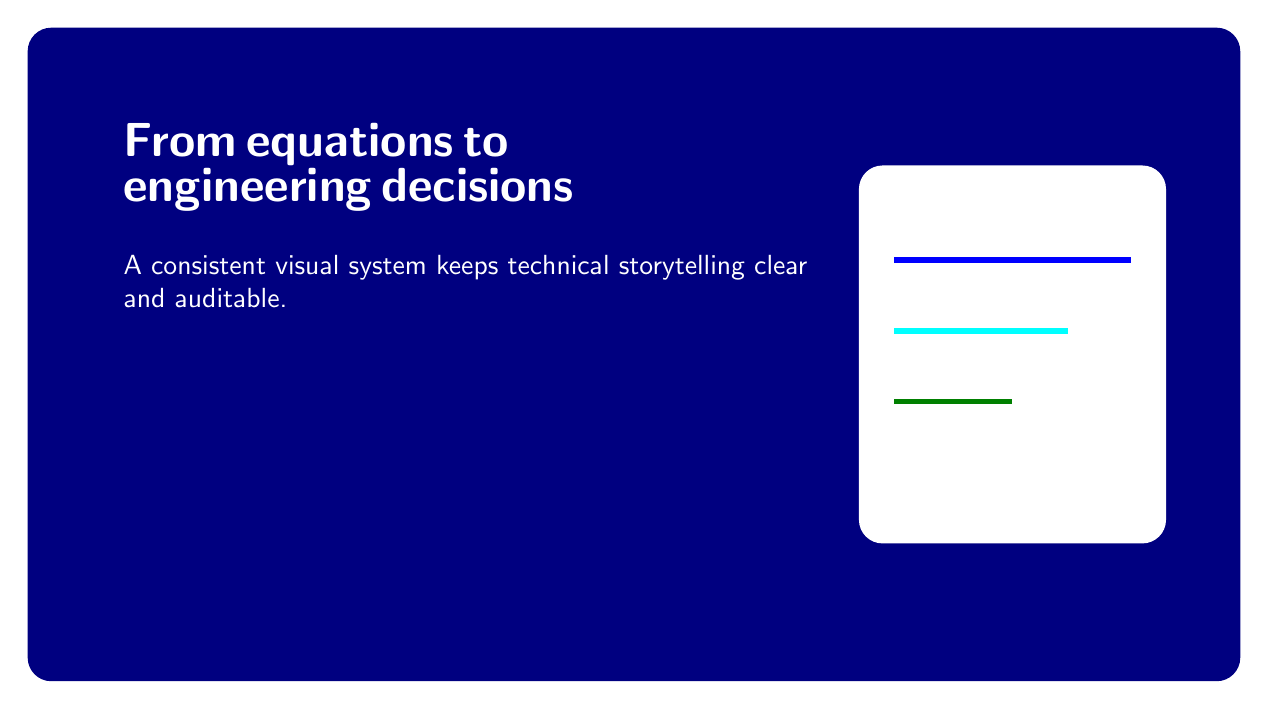
\begin{tikzpicture}
\node[fill=Navy,rounded corners=3mm,minimum width=154mm,minimum height=83mm] (s) {};
\node[anchor=north west,text width=90mm] at ([xshift=11mm,yshift=-11mm]s.north west) {{\sffamily\bfseries\fontsize{19}{22}\selectfont\color{White}From equations to\\engineering decisions}\par\vspace{5mm}{\sffamily\fontsize{10}{14}\selectfont\color{White!80}A consistent visual system keeps technical storytelling clear and auditable.}};
\node[rounded corners=3mm,fill=White,minimum width=39mm,minimum height=48mm] at ([xshift=-29mm]s.east) {};
\draw[Blue,line width=2pt] ([xshift=-44mm,yshift=12mm]s.east)--([xshift=-14mm,yshift=12mm]s.east);
\draw[Cyan,line width=2pt] ([xshift=-44mm,yshift=3mm]s.east)--([xshift=-22mm,yshift=3mm]s.east);
\draw[Green,line width=2pt] ([xshift=-44mm,yshift=-6mm]s.east)--([xshift=-29mm,yshift=-6mm]s.east);
\end{tikzpicture}
\end{center}
\vspace{8mm}
\begin{center}\pill{STRUCTURED STORY}\quad\pill{SPEAKER NOTES}\quad\pill{REUSABLE SECTIONS}\quad\pill{DESIGN REVIEW READY}\end{center}
\end{minipage}\slidefooter
\newpage

%6 ieee
\pagecolor{Mist}\setslide{6}
\vspace*{18mm}\hspace*{16mm}\begin{minipage}{184mm}
\slideheading{Enhanced IEEE Paper Template}{A complete two-column example demonstrating equations, figures, tables, citations, and bibliography management.}
\vspace{7mm}
\begin{minipage}[t]{92mm}
\begin{tikzpicture}
\node[fill=White,draw=Line,minimum width=80mm,minimum height=108mm] (p) {};
\node[font=\sffamily\bfseries\fontsize{8.5}{10}\selectfont,text=Navy,text width=68mm,align=center] at ([yshift=-10mm]p.north) {A COMPACT REPRODUCIBLE EXAMPLE OF CONVENTIONAL AND MVDR BEAMFORMING};
\foreach \x in {-18,18}{\foreach \y in {-32,-40,-48,-56,-64,-72,-80,-88}{\draw[Line,line width=.7pt] ([xshift=\x mm-14mm,yshift=\y mm]p.north)--([xshift=\x mm+14mm,yshift=\y mm]p.north);}}
\draw[Blue,line width=1.5pt] ([xshift=-32mm,yshift=-94mm]p.north)--([xshift=31mm,yshift=-94mm]p.north);
\end{tikzpicture}
\end{minipage}\hfill
\begin{minipage}[t]{83mm}
\begin{carouselitemize}
\item IEEEtran conference layout
\item Nine numbered equations
\item TikZ workflow diagram
\item External vector beam-pattern figure
\item Two publication-style tables
\item Five cited bibliography records
\end{carouselitemize}
\vspace{5mm}
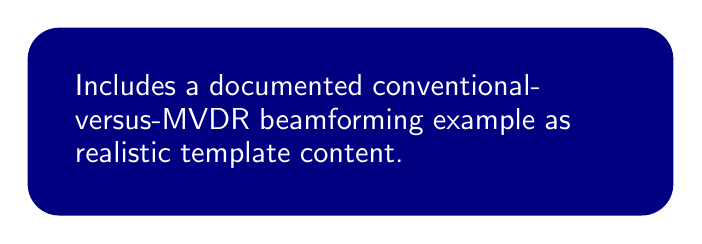
\begin{tikzpicture}
\node[rounded corners=4mm,fill=Navy,inner sep=6mm,text width=70mm,text=White] {\sffamily\fontsize{10.5}{14}\selectfont Includes a documented conventional-versus-MVDR beamforming example as realistic template content.};
\end{tikzpicture}
\end{minipage}
\end{minipage}\slidefooter
\newpage

%7 workflow
\pagecolor{White}\setslide{7}
\vspace*{18mm}\hspace*{16mm}\begin{minipage}{184mm}
\slideheading{Documentation treated as an engineering system}{Meaningful changes are isolated, reviewed, documented, and merged through a repeatable repository workflow.}
\vspace{11mm}
\begin{center}
\begin{tikzpicture}[node distance=7mm, every node/.style={font=\sffamily\bfseries\fontsize{10}{12}\selectfont}]
\node[rounded corners=3mm,fill=Blue!10,draw=Blue!30,minimum width=31mm,minimum height=22mm] (b) {Feature branch};
\node[rounded corners=3mm,fill=Cyan!10,draw=Cyan!35,minimum width=31mm,minimum height=22mm,right=of b] (v) {Validation};
\node[rounded corners=3mm,fill=Green!10,draw=Green!35,minimum width=31mm,minimum height=22mm,right=of v] (h) {Handoff};
\node[rounded corners=3mm,fill=Blue!10,draw=Blue!30,minimum width=31mm,minimum height=22mm,right=of h] (p) {Pull request};
\node[rounded corners=3mm,fill=Navy,text=White,minimum width=31mm,minimum height=22mm,right=of p] (m) {Controlled merge};
\draw[-{Latex[length=2.5mm]},Slate,line width=1pt] (b)--(v);
\draw[-{Latex[length=2.5mm]},Slate,line width=1pt] (v)--(h);
\draw[-{Latex[length=2.5mm]},Slate,line width=1pt] (h)--(p);
\draw[-{Latex[length=2.5mm]},Slate,line width=1pt] (p)--(m);
\end{tikzpicture}
\end{center}
\vspace{13mm}
\begin{center}
\begin{tikzpicture}
\node[rounded corners=4mm,fill=Mist,draw=Line,inner sep=8mm,text width=156mm] {\sffamily\fontsize{13}{18}\selectfont\color{Ink}\textbf{Why it matters:} the repository records not only the final files, but also implementation scope, validation evidence, limitations, rollback guidance, and follow-up work.};
\end{tikzpicture}
\end{center}
\end{minipage}\slidefooter
\newpage

%8 close
\pagecolor{Navy}\setslide{8}
\begin{tikzpicture}[remember picture,overlay]
\fill[Blue] ([xshift=-15mm,yshift=-25mm]current page.north east) circle (45mm);
\node[anchor=north west,text width=170mm] at ([xshift=22mm,yshift=-37mm]current page.north west) {{\sffamily\bfseries\fontsize{29}{33}\selectfont\color{White}Built for engineering work\\that needs to be understood,\\reviewed, and reused.}\par\vspace{9mm}{\sffamily\fontsize{13}{18}\selectfont\color{White!82}Academic projects \textbullet\ Research reports \textbullet\ Design reviews\\Technical consulting \textbullet\ Reproducible engineering workflows}};
\node[rounded corners=4mm,fill=White,minimum width=170mm,minimum height=35mm] at ([yshift=-42mm]current page.center) {};
\node[text width=150mm,align=center] at ([yshift=-42mm]current page.center) {{\sffamily\bfseries\fontsize{13}{16}\selectfont\color{Navy}Explore the repository}\\[2mm]{\sffamily\fontsize{10.5}{13}\selectfont\color{Blue}github.com/hmolhem/engineering-latex-templates}};
\node[anchor=south west,text=White] at ([xshift=22mm,yshift=31mm]current page.south west) {\sffamily\bfseries\fontsize{11}{13}\selectfont Hossein Molhem};
\node[anchor=south east,text=White!80] at ([xshift=-22mm,yshift=31mm]current page.south east) {\sffamily\fontsize{9}{11}\selectfont Engineering documentation \textbullet\ RF \textbullet\ Antennas};
\end{tikzpicture}
\end{document}
